\documentclass[journal,12pt,twocolumn]{IEEEtran}
\usepackage{tikz}
\usepackage{amsmath}
\usepackage{breqn}
\usepackage{amssymb}
\pagestyle{empty}
\usepackage{setspace}
\usepackage{gensymb}
\singlespacing

\usepackage{amsmath}
\usepackage{amsthm}
\begin{document}
\newcommand{\myvec}[1]{\ensuremath{\begin{pmatrix}#1\end{pmatrix}}}
\newcommand{\cmyvec}[1]{\ensuremath{\begin{pmatrix*}[c]#1\end{pmatrix*}}}
\providecommand{\norm}[1]{\lVert#1\rVert}
\newcommand{\mydet}[1]{\ensuremath{\begin{vmatrix}#1\end{vmatrix}}}
\providecommand{\sbrak}[1]{\ensuremath{{}\left[#1\right]}}
\providecommand{\lsbrak}[1]{\ensuremath{{}\left[#1\right.}}
\providecommand{\rsbrak}[1]{\ensuremath{{}\left.#1\right]}}
\providecommand{\brak}[1]{\ensuremath{\left(#1\right)}}
\providecommand{\lbrak}[1]{\ensuremath{\left(#1\right.}}
\providecommand{\rbrak}[1]{\ensuremath{\left.#1\right)}}
\providecommand{\cbrak}[1]{\ensuremath{\left\{#1\right\}}}
\providecommand{\lcbrak}[1]{\ensuremath{\left\{#1\right.}}
\providecommand{\rcbrak}[1]{\ensuremath{\left.#1\right\}}}
\let\StandardTheFigure\thefigure
\let\vec\mathbf

\title{
Assignment - 2
}
\author{ Soham Bhatt \\SM21MTECH14004}
\maketitle
\newpage
\bigskip
\bibliographystyle{IEEEtran}
\section*{\textbf{Problem}}
\noindent
\textbf{\textsl{1. Find the in-center of the triangle formed by the following points lie,}}
$$$$
\textbf{\textsl{i. 5x-12y=0,\quad ii. 5x+12y+60=0,\quad iii. 5x+12y-60=0}}
\noindent
\section*{\textbf{Solution}}
\noindent
First, we need to find the intersection point of given three lines, \\
\\
Let's find the intersection of line (i) and (ii),\\
\\
Let's write it in AX = B form,\\

\myvec{X_1&Y_1\\X_2&Y_2}\myvec{X\\Y} = \myvec{C_1\\C_2}\\
\\

\myvec{5&-12\\5&12}\myvec{X_1\\Y_1} = \myvec{0\\-60}\\
\\
By solving above equation, we are getting the intersection point of line (i) and (ii),\\
Let's call it as M:
\\

M = \myvec{X_1\\Y_1} = \myvec{-6\\-2.5} \qquad (1)\\
\\
In the same way, intersection of line (ii) and (iii) is,\\
\\

\myvec{5&12\\12&5}\myvec{X_2\\Y_2} = \myvec{-60\\60}\\
\\
By solving above equation, we are getting the intersection point of line (ii) and (iii),\\
Let's call it as N:
\\

N = \myvec{X_2\\Y_2} = \myvec{8.571\\-8.571} \qquad (2)\\
\\
In the same way, intersection of line (i) and (iii) is,\\
\\

\myvec{5&-12\\12&-5}\myvec{X_3\\Y_3} = \myvec{0\\60}\\
\\
By solving above equation, we are getting the intersection point of line (i) and (iii),\\
Let's call it as O:
\\

O = \myvec{X_3\\Y_3} = \myvec{4.260\\1.775} \qquad (3)\\
\\
Now we need to find difference between each vectors,\\

Difference between vectors N and O:\\
\\
N = \myvec{8.571\\-8.571}, O = \myvec{4.260\\1.775}\\
\\
0-N = \myvec{-4.311\\10.345}\\
\norm{\vec{O}-\vec{N}} = \sqrt{(-4.311^2 + 10.345^2)}\\
\norm{\vec{O}-\vec{N}} = 11.207 \qquad\qquad (\vec{D_1})\\

Difference between vectors M and O:\\
\\
M = \myvec{-6\\-2.5}, O = \myvec{4.260\\1.775}\\
\\
0-M = \myvec{10.26\\4.275}\\
\norm{\vec{O}-\vec{M}} = \sqrt{(10.260^2 + 4.275^2)}\\
\norm{\vec{O}-\vec{M}} = 11.115 \qquad\qquad (\vec{D_2})\\
\\

Difference between vectors M and N:\\
\\
M = \myvec{-6\\-2.5}, N = \myvec{8.571\\-8.571}\\
\\
N-M = \myvec{14.571\\-6.071}\\
\norm{\vec{N}-\vec{M}} = \sqrt{(14.571^2 + 6.071^2)}\\
\norm{\vec{N}-\vec{M}} = 15.785 \qquad\qquad (\vec{D_3})\\
\\

Formula for finding in-center (I) of triangle with three given coordinates is,\\
$$ \bigg(\frac{D_1X_1 + D_2X_2 + D_3X_3}{D_1+D_2+D_3} ,\quad\frac{D_1Y_1 + D_2Y_2 + D_3Y_3}{D_1+D_2+D_3}\bigg) $$
\\
By putting all the values,\\
$$ \bigg(\frac{(11.207)(-6) + (11.115)(8.571) + (15.785)(4.260)}{11.207+11.115+15.785} ,$$
$$\quad\frac{(11.207)(-2.5) + (11.115)(-8.571) + (15.785)(1.775)}{11.207+11.115+15.785}\bigg) $$
\\ \\
I = \myvec{2.500\\-2.499}

\begin{figure}[!ht]
    \centering
    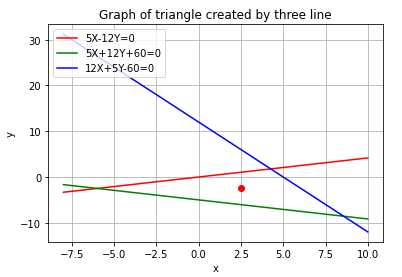
\includegraphics[width=\columnwidth]{graph.png}
    \caption{Triangle created by three lines}
    \label{fig:}
\end{figure}

\end{document}